\chapter{Performance}
\label{ch:performance} % 2000-2500 words

As enumerated in the objectives summary section of the introduction \ref{ch:ssec:objectives-summary}, on of the three requirements for Rust's suitability as a language for High-Performance Computing is having a comparable performance to C++, one of the most commonly used languages in current usage.

This chapter provides an empirical assessment of the performance of the Rust translation of the HPCCG mini-app. As discussed in the background section introducing HPCCG \ref{ssec:hpccg}, this is representative of High-Performance Computing workloads, due to the design goals of Mantevo Suite mini-apps being representative of full applications to facilitate hardware-software co-design. We leverage this property to instead assess the Rust language's suitability for such workloads by comparing the performance of the Rust translation to the original C++ implementation.

This performance profiling will begin with the use of instrumentation tooling to identify hot-spots in source code, characterising the bottlenecks in the Rust and C++ compiled executables. This allows a direct comparison of compiled assembly, yielding a clear picture of ways in which the Rust language differs from C++. Then, the HPC MultiBench tool will be used to run and analyse direct measurements of the Rust and C++ codebases. This allows the characterisation and comparison of performance for strong and weak scaling, and parallelism approaches, along with the generation of roofline models.

\section{Profiling tools}
\label{sec:profiling-tools} % 500 words

Software profilers are a category of tools which are used to measure properties of running programs. They differ from static analysis tools, as they analyse programs dynamically as they run, usually through instrumentation inserted at compile time, rather than using the source code itself. Profilers are most often used to characterise the performance and memory usage of programs, and through instrumentation can identify ``hotspots'' -- code sections in the program which account for a disproportionate amount of the metric, such as overall runtime. This makes profilers useful for guiding optimisations, as engineering effort can be targeted at the portion of program which impacts performance most greatly.

Performance profilers can also be used to compare implementations of the same software in different languages. Comparing the  profiles of the programs on the same problem size can elucidate where one language loses performance over another, and give insights into key factors such as vectorisation and memory bandwidth utilisation.

We choose to use a variety of performance profilers, because some profilers provide many more metrics and analysis options, but typically at the expense of the simple and ergonomic user interface. As a result of this, we used \texttt{perf} for the majority of profiling tasks, as they provide a convenient command line interface for instrumentation statistical sampling. We also used the Intel\textregistered\ oneAPI\texttrademark\ suite of tools, including Intel\textregistered\ vTune\texttrademark and Intel\textregistered\ Advisor\texttrademark, as these provide a vast array of capabilities such as roofline analysis, but with a complex graphical-only interface.


\subsection{The \texttt{perf} profiler}
\label{ssec:perf profiler}

\texttt{perf} is 

The \texttt{perf} profiler was used throughout the translation process to identify hotspots in the code. The benefit of this process was two-fold. Firstly, it allowed manual performance-guided optimisation, allowing prioritisation of engineering effort to ensure the Rust implementation was a fair representation of the full extent of the languages capabilities when comparing it to C++. Secondly, the hotspots identified provided a strong insight into the parts of Rust programs that fall short of C++, which informs the assessment of the suitability of Rust for High-Performance computing applications.

% As discussed in the introduction
The Rust programming language places a strong focus on the prevention of undefined behaviour, including enforcing memory and thread safety. The key insight of the language was that many of these guarantees against undefined behaviour can be made at compile time, through the ownership model enforced by the borrow checker. However, there is not enough information at compile time to fully guarantee these characteristics. For example, creating a vector of a length provided by user input at run time is a common operation within many programs. However, if the programmer accesses this vector by a fixed index in the source code, the compiler cannot guarantee the indexing operation is within the bounds of this vector, since its size is not known until runtime. To avoid undefined behaviour, Rust checks the bounds of every indexing operations to guarantee that the index is not out of range, but this incurs a performance cost -- roughly doubling the time taken for vector indexing. To avoid this check in performance critical applications when the bounds are already guaranteed, Rust provides the \mintinline{rust}{get_unchecked} function, which does not perform the bound check. This performance cost can be seen through comparing \texttt{perf} reports when using the default bounds checked indexing in Figure \ref{fig:perf-checked}, against unchecked indexing in Figure \ref{fig:perf-unchecked}.

\begin{figure}[H]
    \centering
    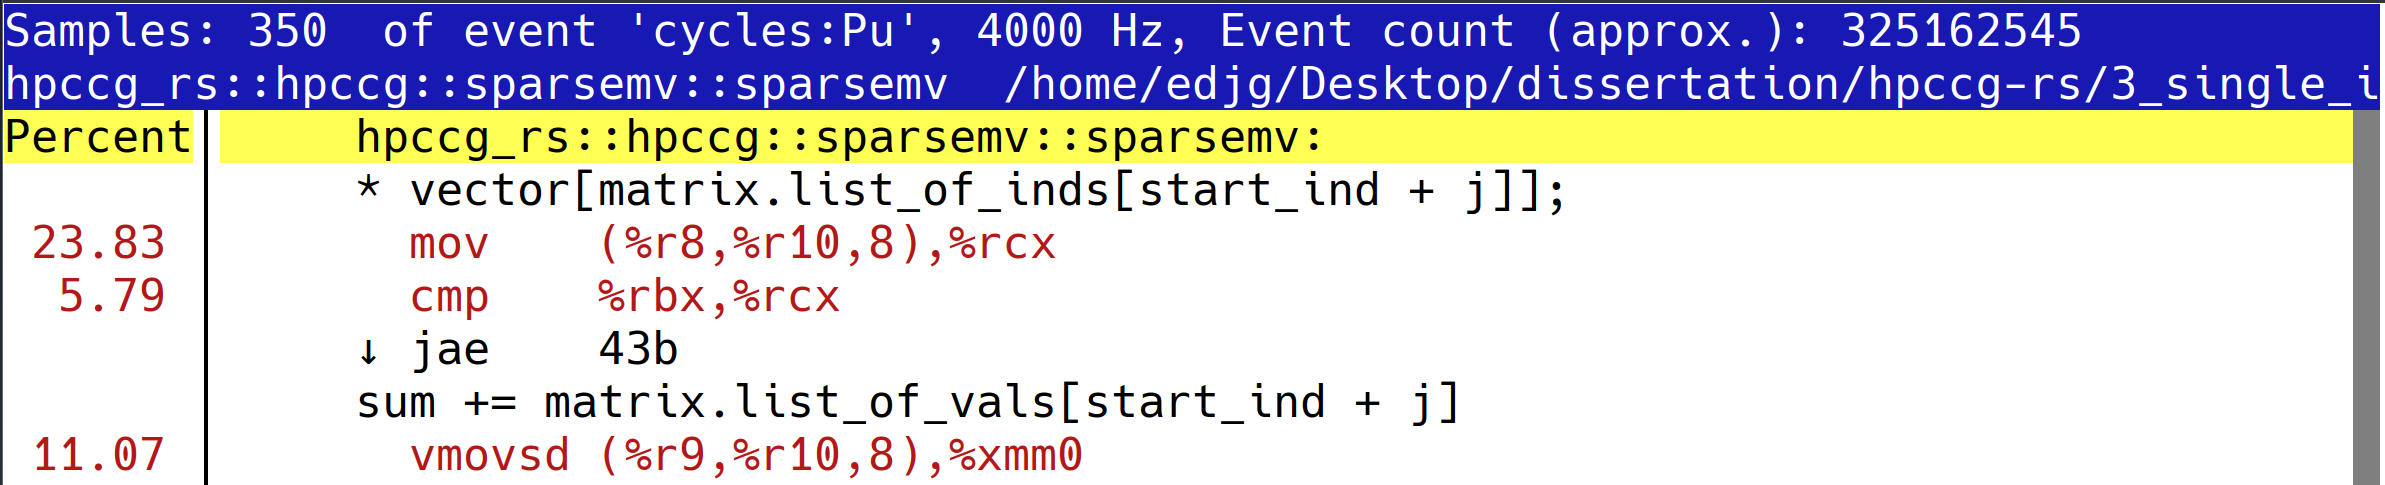
\includegraphics[width=0.95\textwidth]{images/5_performance/perf_checked_op.png}
    \caption{A screenshot of the \text{perf} report of a Rust translation of HPCCG using the default checked indexing.}
    \label{fig:perf-checked}
\end{figure}

\begin{figure}[H]
    \centering
    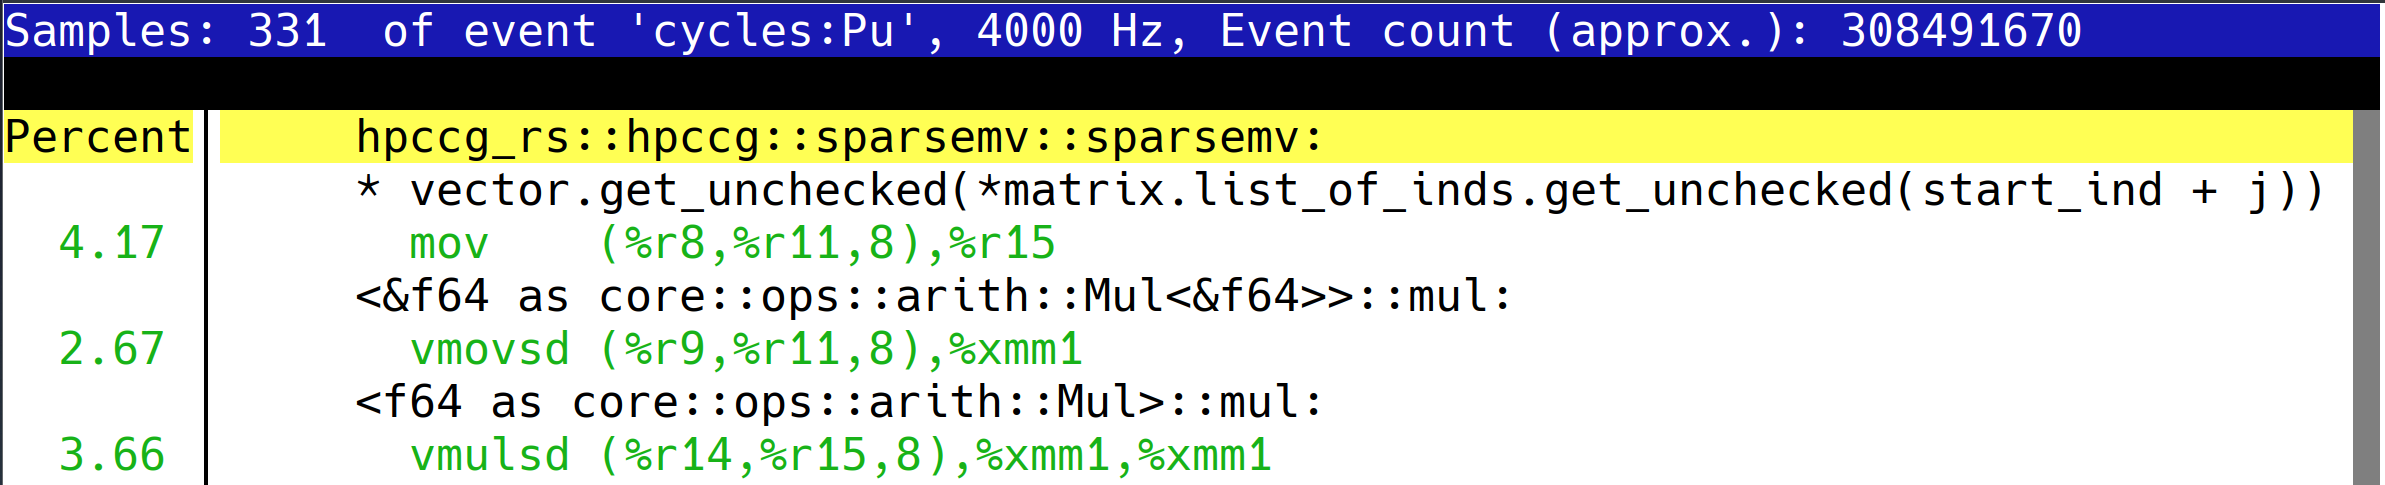
\includegraphics[width=0.95\textwidth]{images/5_performance/perf_unchecked_op.png}
    \caption{A screenshot of the \text{perf} report of a Rust translation of HPCCG using the unchecked indexing.}
    \label{fig:perf-unchecked}
\end{figure}

From these figures, we can see that the the bounds checking operation dominate the total runtime of the program, with $23.83 + 5.79 = 29.62$ percent of the runtime being taken up by the \mintinline{rust}{vector[matrix.list_of_inds[start_ind + j]]} operation in the bounds checked version, but only $4.17 + 2.67 + 3.66 = 10.5$ percent in the version without bounds checking. The empirical result of a $2.82\times$ speed-up for array indexing, a very common operation in High-Performance computing workloads, demonstrates the utmost importance of understanding and leveraging the full extent of the Rust language to be able to write performant software.


% Zero-cost abstractions
% iterators as a zero-cost abstraction? are they?

\subsection{The Intel\textregistered\ oneAPI\texttrademark\ suite}
\label{ssec:perf profiler}
% Intel vTune Advisor
% Roofline model


Performance profilers provide a very powerful tool for identifying and optimising away hotspots in running programs. However, profilers are typically best suited for measuring many performance metrics in a fixed configuration, such as with a set number of processor threads and MPI ranks. To assess Rust's suitability for High-Performance Computing, we only needed a few metrics such as runtime and FLOPs, but wanted to measure how these varied across a wide range of metrics, with statistical confidence. As a result of this, we switched to a direct measurement approach driven by the HPC MultiBench tool, which was designed for this purpose.

\section{Direct measurement}
\label{sec:direct-measurement} % 2000 words

For Rust to be a suitable language for High-Performance Computing workloads, it must have a comparable performance across both a range of parallelism approaches, from serial execution to multi-threading and message passing across a compute cluster, and for large data volumes. To assess this, we used a wall clock approach to time the original C++ and the translated Rust implementations of HPCCG across a variety of problem sizes, and with a variety of thread counts and MPI sizes.

\subsection{Experimental methodology}
\label{ssec:experimental-methodology}

% In the intro to the book Performance Tuning of Scientific Applications, David Bailey suggests nine guidelines for presenting performance results without misleading the reader. Paraphrasing only slightly, these are: 

\subsubsection{System specifications}
\label{sssec:system-specifications}

During the course of experimentation, three different compute resources were used: Athena, the author's personal laptop; Kudu, the DCS batch compute system; and Avon, the Warwick SCRTP High-Performance Computing resource. Athena was used for the translation effort and initial testing, but not for any experimental results. However, since tests during the development process informed decisions made during the design process, its system specifications are relevant. Kudu was used for the majority of testing and the project presentation demo, as it is easy to access and has short queue times. Avon was used for later tests to confirm results, and for very large tests which exceeded Kudu's capacity.

Allow for reproducibility of the reported test data, the hardware specifications for the machines used as follows, with the results of \texttt{lscpu} for the machines are listed in Appendix \ref{sec:hardware-specifications} for completeness.

\begin{itemize}
    \item Athena has a \texttt{Intel(R) Core(TM) i7-8565U CPU @ 1.80GHz} with eight logical cores.
    \item Kudu has a \texttt{Intel(R) Xeon(R) CPU E5-2660 v3 @ 2.60GHz} with 40 logical cores.
    \item Avon has a \texttt{Intel(R) Xeon(R) Platinum 8268 CPU @ 2.90GHz} with 48 logical cores.
\end{itemize}

The \texttt{lstopo} tool can be used to draw a graphical representation of both the hardware composing the system, and its topology. This gives a further insight into the hardware being used to run the tests, beyond the CPU model. Figures \ref{fig:athena-topology}, \ref{fig:kudu-topology} and \ref{fig:avon-topology} show the hardware topologies of the Athena, Kudu, and Avon systems respectively. For Kudu and Avon, \texttt{slurm} is used to dispatch jobs, so the commands are run from within a \texttt{slurm} job to be representative of the compute nodes rather than the login nodes of the cluster.

\begin{figure}[H]
    \centering
    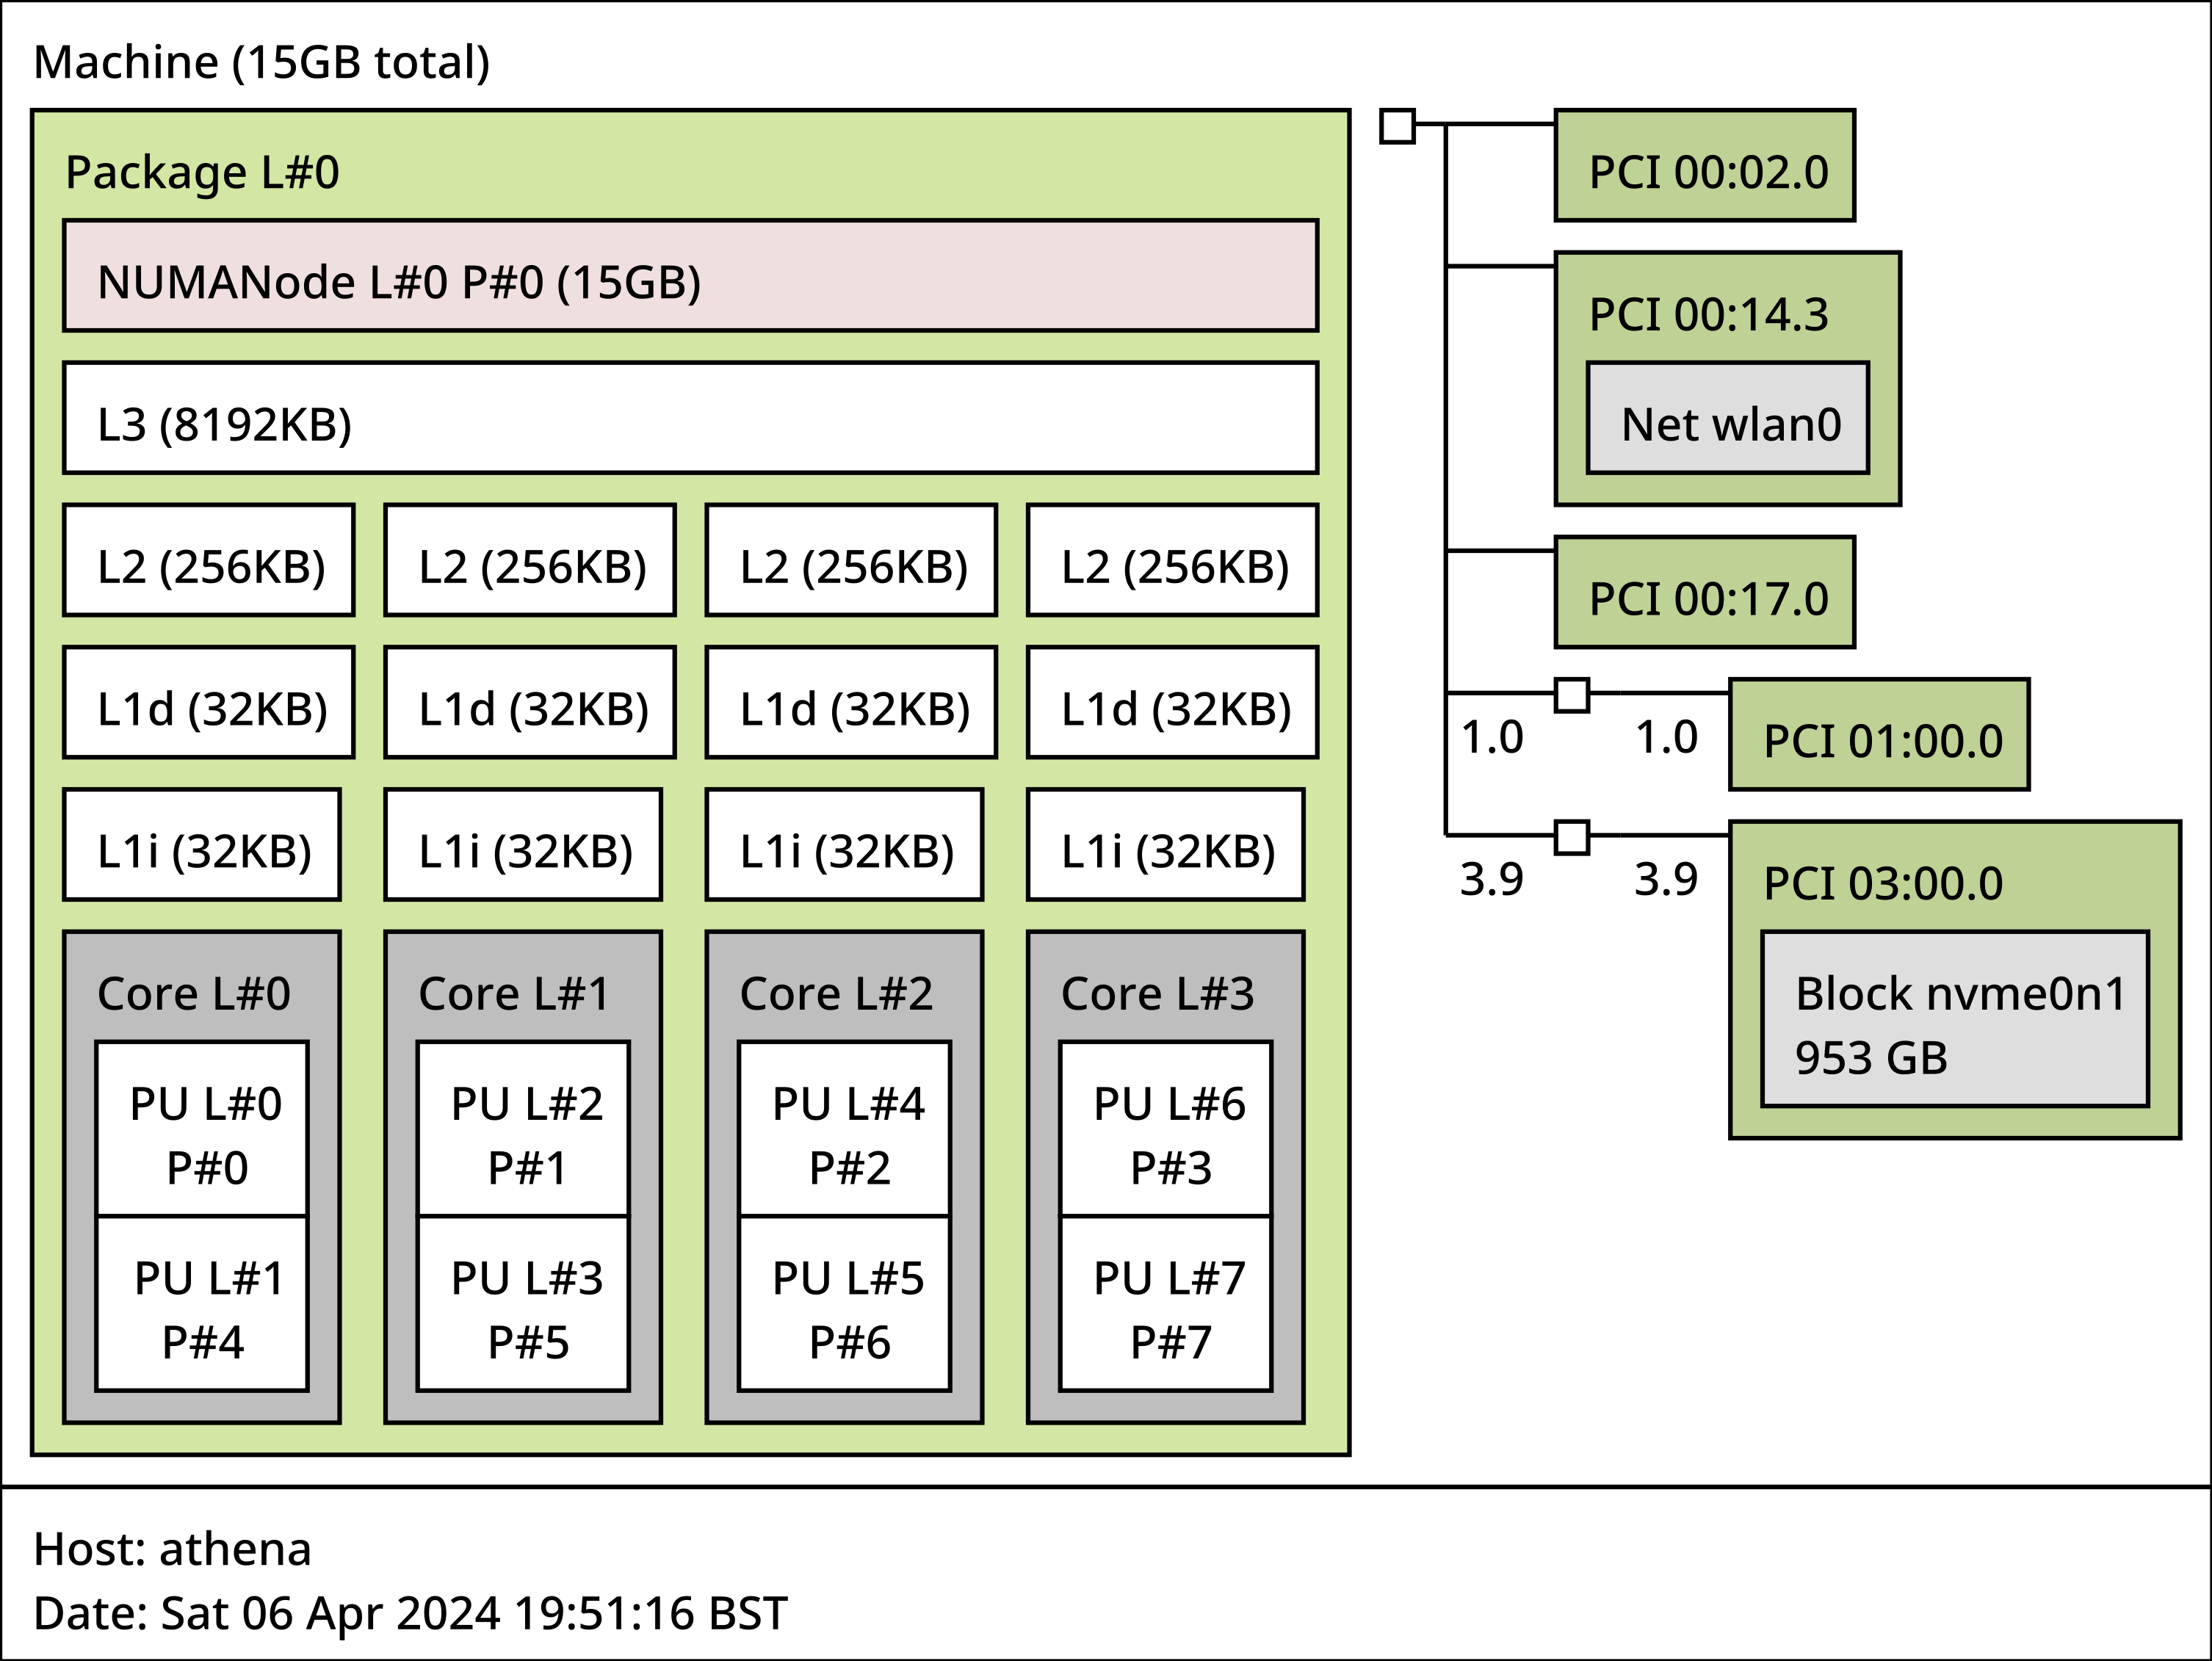
\includegraphics[width=0.75\textwidth]{images/5_performance/athena-topology.png}
    \caption{A diagram of a hardware topology of Athena.}
    \label{fig:athena-topology}
\end{figure}

\begin{figure}[H]
    \centering
    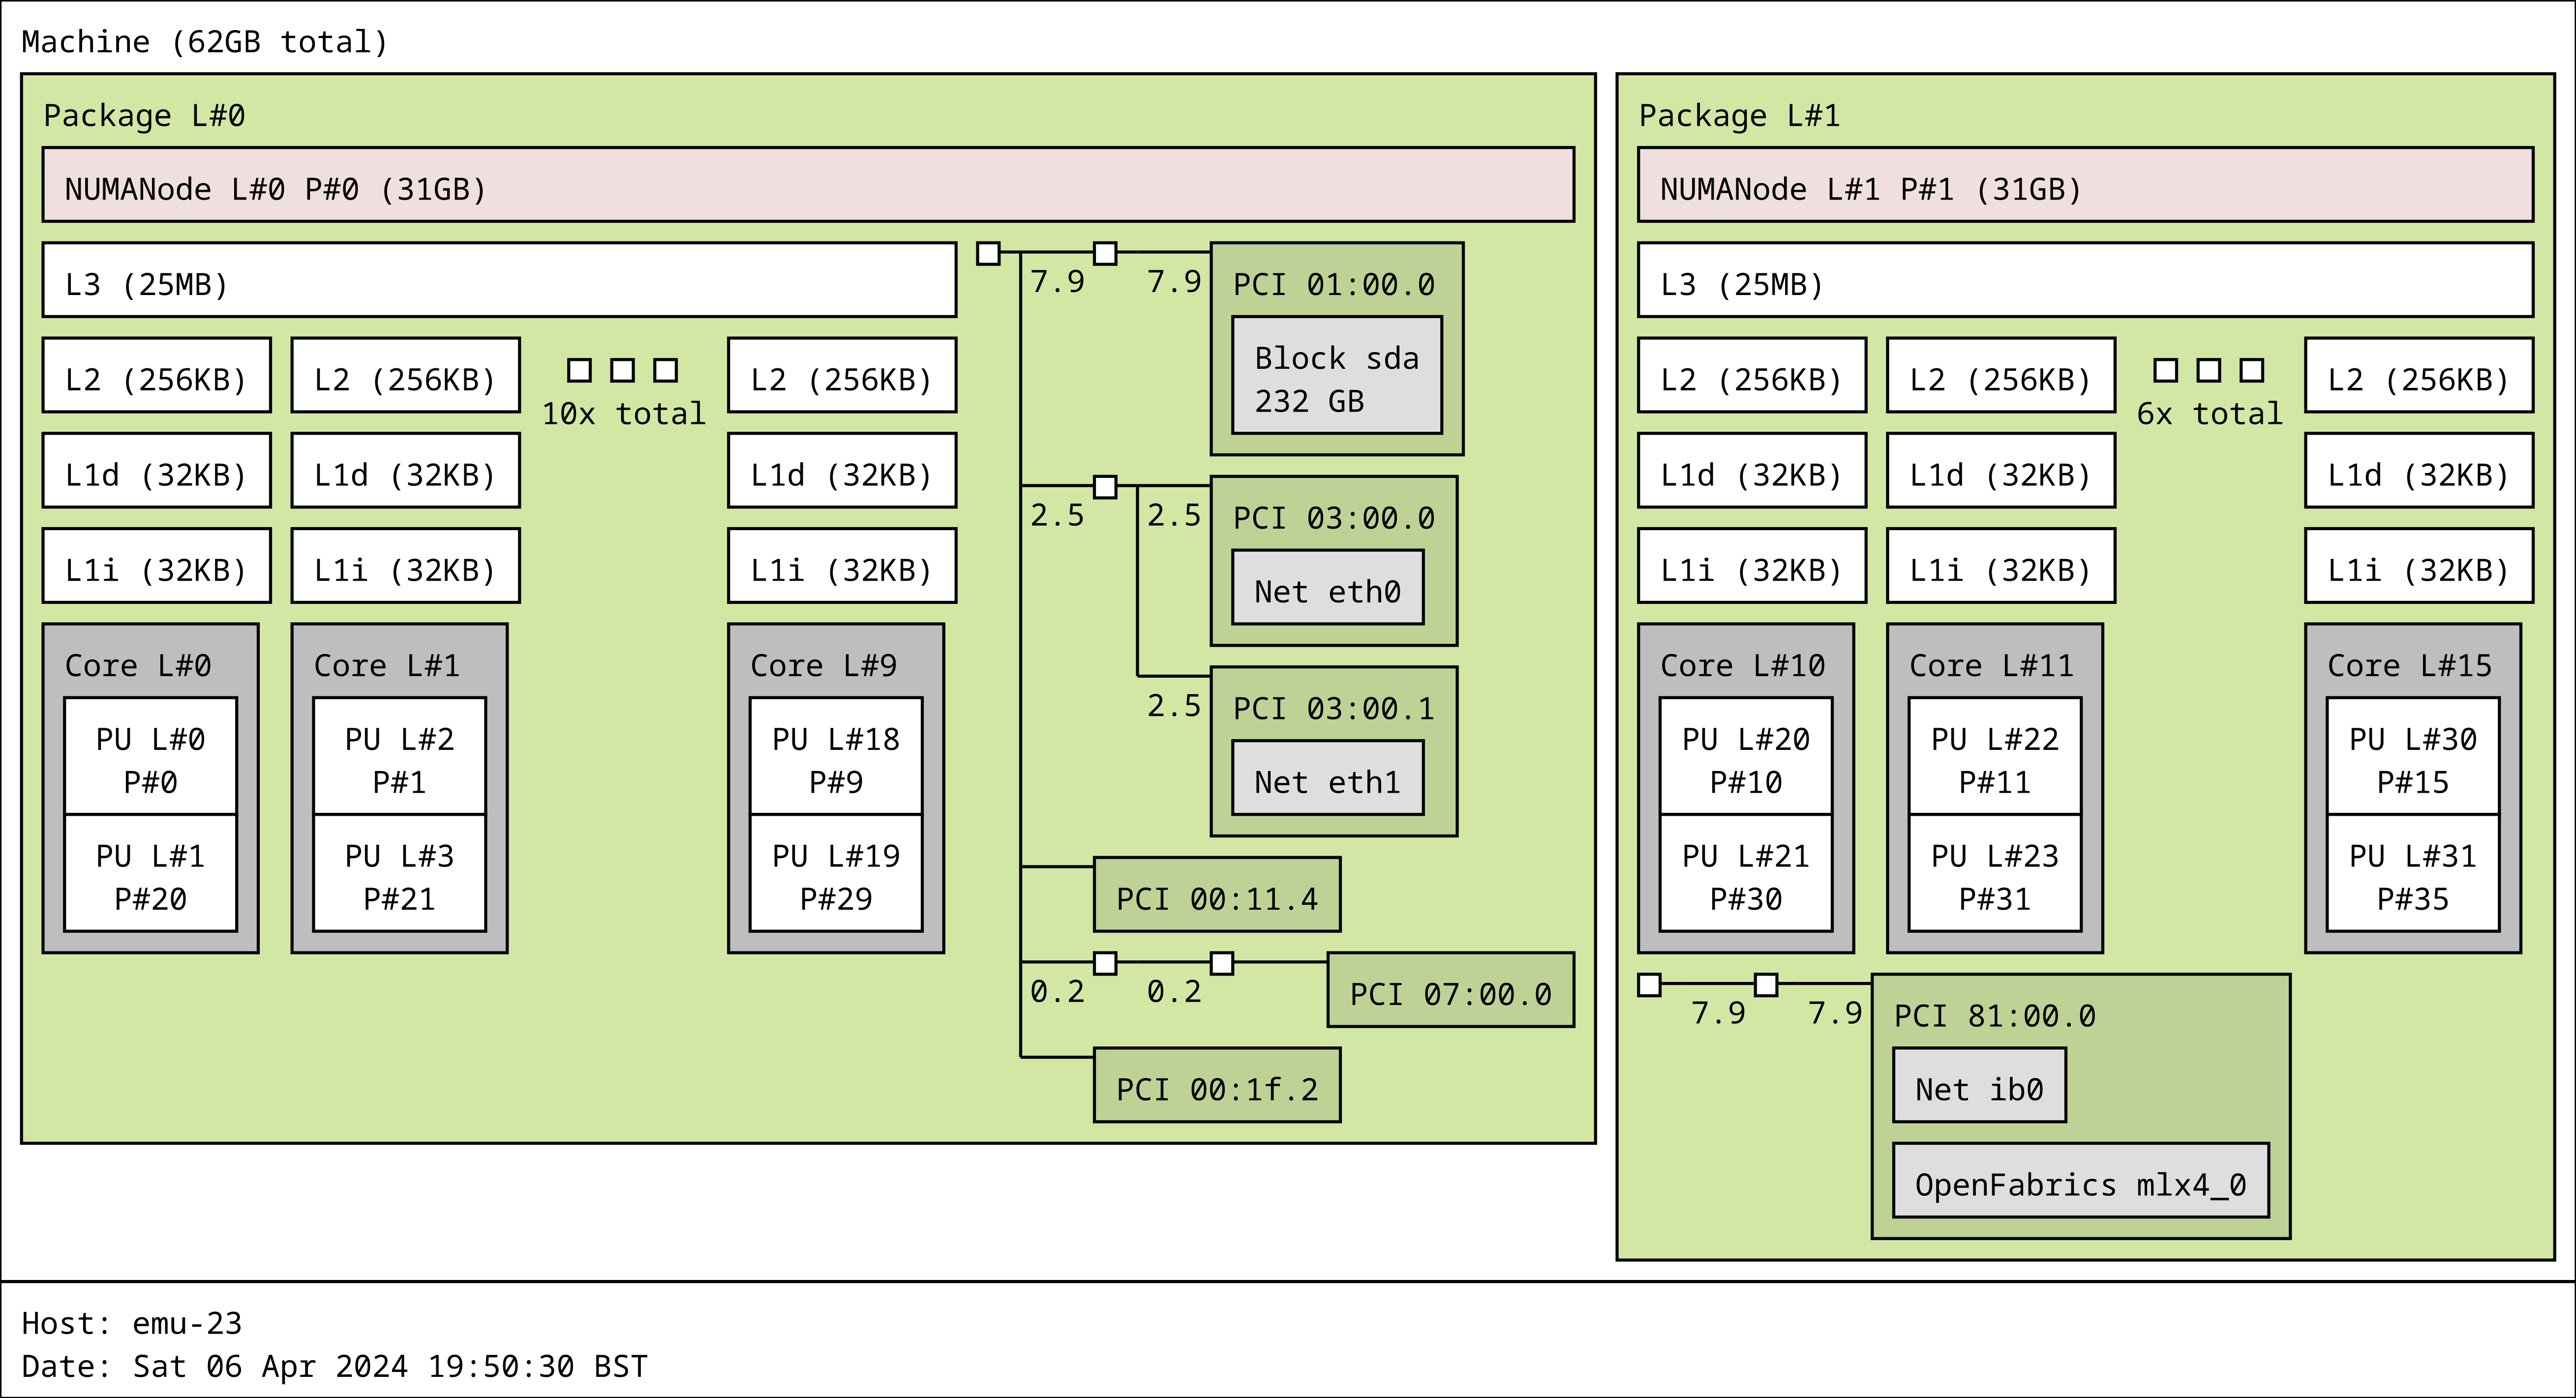
\includegraphics[width=0.85\textwidth]{images/5_performance/kudu-topology.png}
    \caption{A diagram of a hardware topology of Kudu.}
    \label{fig:kudu-topology}
\end{figure}

\begin{figure}[H]
    \centering
    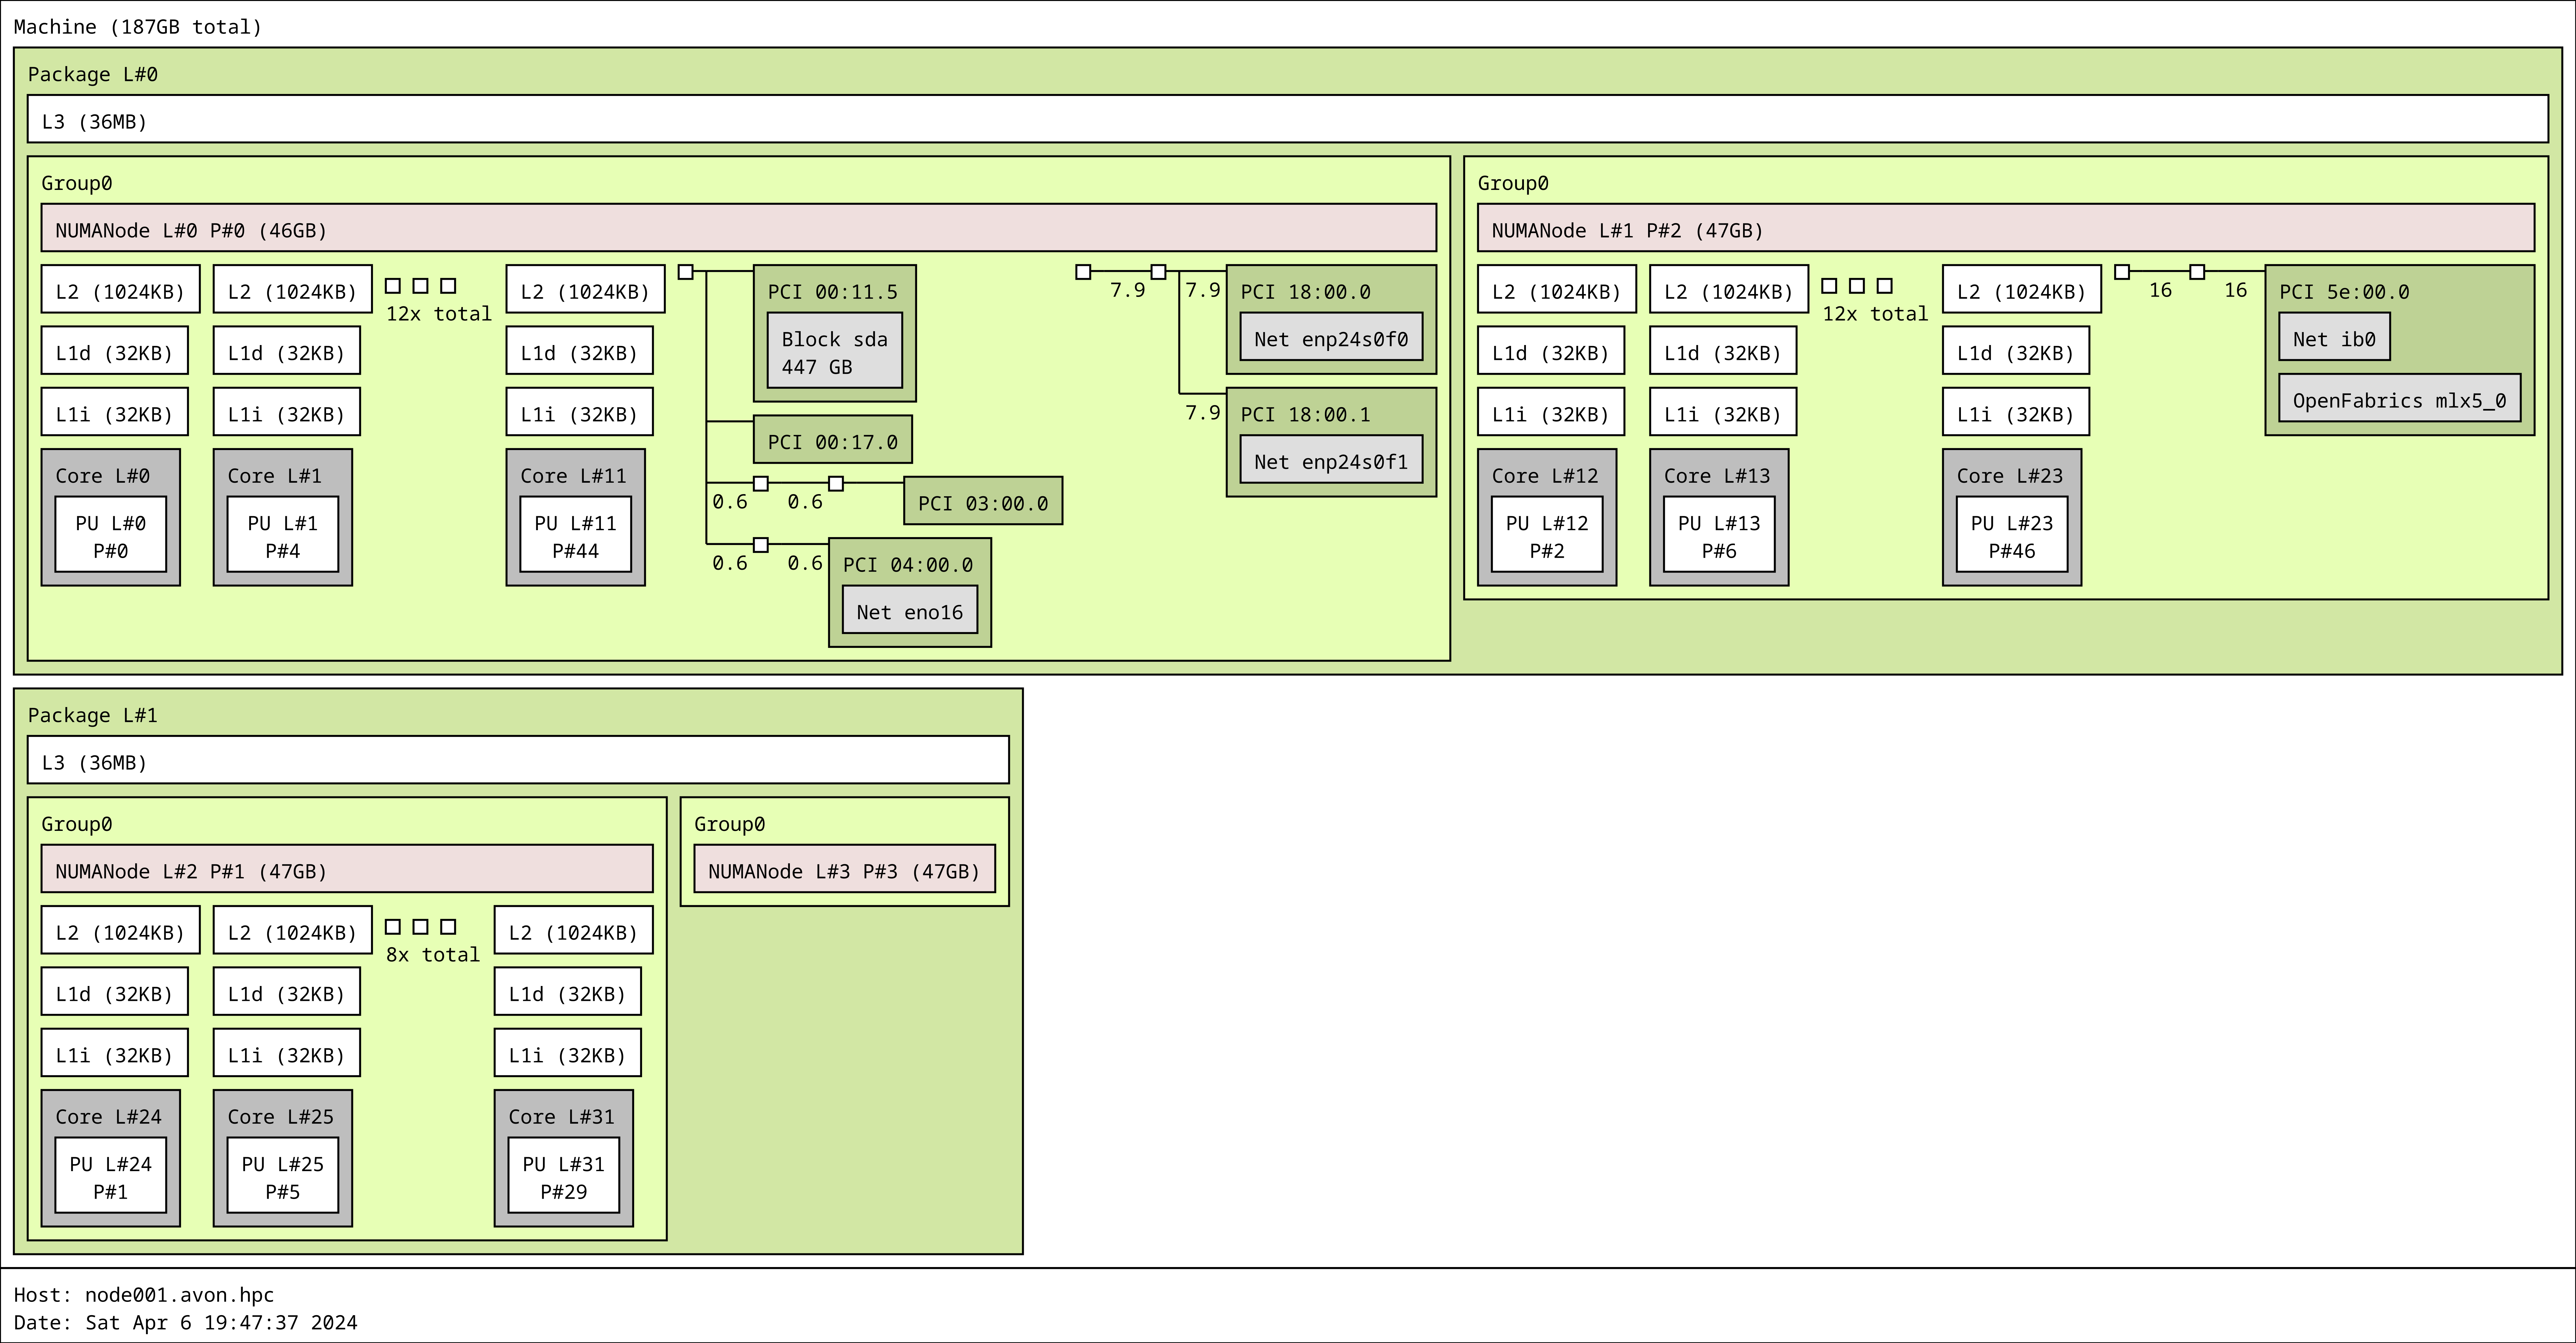
\includegraphics[width=0.95\textwidth]{images/5_performance/avon-topology.png}
    \caption{A diagram of a hardware topology of Avon.}
    \label{fig:avon-topology}
\end{figure}

The software versions used for benchmarking across the three systems are enumerated in the following table:

\begin{table}[H]
    \caption{A table showing the software versions across the three compute resources.}
    \label{table:perfTools}
    \begin{tabular}{|p{0.24\linewidth}||p{0.2\linewidth}|p{0.2\linewidth}|p{0.2\linewidth}|}
    \hline
    \textbf{Software name} & \textbf{Athena} & \textbf{Kudu} & \textbf{Avon} \\
    \hline\hline
    Operating system & EndeavourOS 2023.03.26 & Rocky Linux 8.9                & CentOS Linux 8.4.2105          \\\hline
    Linux kernel     & 6.6.24-1-lts                     & 4.18.0-513.18.1. el8\_9.x86\_64 & 4.18.0-305.88.1. el8\_4.x86\_64 \\\hline
    rustc            & 1.73.0                           & 1.75.0                         & 1.75.0                         \\\hline
    clang            & 17.0.6                           & 16.0.6                         & 13.0.1                         \\\hline
    g++              & 13.2.1                           & 9.2.0                          & 11.3.0                         \\\hline
    OpenMP           & 4.5                              & 4.5                            & 4.5                            \\\hline
    rayon            & 1.8.0                            & 1.8.0                          & 1.8.0                          \\\hline
    Open MPI         & 5.0.2                            & 4.0.5                          & 4.1.4                          \\\hline
    rs-mpi           & 0.7.0                            & 0.7.0                          & 0.7.0                         \\\hline
    \end{tabular}
\end{table}


\subsection{Strong scaling}
\label{ssec:strong-scaling}

% What is strong scaling
Patterson and Hennessy define strong scaling as ``measuring the speed-up [due to parallelisation] while keeping the problem size fixed'' \cite{pattersonHennessyComputerOrganisationArchitecture}. This can be measured by recording the wall clock time taken for a fixed problem, whilst varying the degree of parallelisation, given by number of threads or MPI ranks. It can be used to show how adding more computational resources to a problem effects its performance. A perfect speedup due to parallelisation would decrease execution time linearly with the number of resources added. However, programs with a serial component cannot achieve this perfect speed-up as a corollary of Amdahl's law \cite{amdahlsLaw}:

\begin{equation}
    S = \frac{1}{f + \frac{1-f}{P}}
\end{equation}

Where $f$ denotes the proportion of execution time spent on the serial component, $P$ the degree of parallelisation, and $S$ the total speedup of the system as a result of parallelisation. For problems well-suited to parallelisation, we expect to see strong speedup approach the upper bound for performance following Amdahl's law.

% Strong scaling applied to HPCCG
In the context of HPCCG, strong scaling can be measured for single-node (multi-threading only) and multi-node (multi-threading and message passing). The below figures compare the results of the C++ and Rust implementations for strong scaling across single-node and multi-node approaches.

% Figure single node

% Figure multi-node

% Summary

The YAML file which defines this set of runs in the HPC MultiBench tool can be found in Appendix  \ref{}, along with the raw results of the test runs in Appendix \ref{}.

\subsection{Weak scaling}
\label{ssec:weak-scaling}

% What is weak scaling
Patterson and Hennessy define weak scaling as ``measuring the speed-up while keeping the problem size fixed'' \cite{pattersonHennessyComputerOrganisationArchitecture}. This can be measured by recording the wall clock time taken, whilst varying the problem size at the same rate as the varying the degree of parallelisation, given by number of threads or MPI ranks. Since the workload grows with the number of resources added, perfect weak scaling is when the execution time remains constant as both factors are increased.

% Gustafson’s Law 
Unlike strong scaling, we cannot apply Amdahl's law to characterise weak scaling, since it assumes a fixed problem size. Instead, 


% Strong scaling applied to HPCCG
In the context of HPCCG, weak scaling can again be measured for single-node (multi-threading only) and multi-node (multi-threading and message passing). The below figures compare the results of the C++ and Rust implementations for weak scaling across single-node and multi-node approaches.

% Figure single node
% Consider switching to just MPI or just Threading?

% Figure multi-node
% Consider just MPI or both?

% Summary

The YAML file which defines this set of runs in the HPC MultiBench tool can be found in Appendix  \ref{}, along with the raw results of the test runs in Appendix \ref{}.

\subsection{Parallelism approaches}
\label{ssec:parallelism-approaches}

% TODO: cite
In modern High-Performance Computing systems, the majority of performance is achieved through parallelism. As a result of this, for Rust to be suitable for use in High-Performance Computing workloads, it must be able to achieve parallel compute performance similar to that of currently used languages, like C++. This section provides an empirical analysis of the performance of Rust as compared with C++ for increasingly parallel workloads, from serial as a reference to shared memory parallelism through multi-threading and distributed memory parallelism through message passing.

\subsection{Serial execution}
\label{ssec:multi-threaded}

Before exploring various parallelism approaches, it is important to measure a point of reference, in the form of serial execution of the program.

\subsection{Multi-threading}
\label{ssec:multi-threaded}

\subsection{Single node MPI}
\label{ssec:single-node-mpi}

\subsection{Multi-node MPI}
\label{ssec:multi-node-mpi}

\subsection{Performance portability frameworks}
\label{ssec:performance-portability-frameworks}



\section{Roofline models}
\label{sec:roofline-models}

% Introducing roofline models
% Using Intel Advisor
% Using HPC multibench


\section{Summary of results}
\label{sec:performance-results}